\documentclass[12pt]{article}

\usepackage[style=authoryear]{biblatex}
\addbibresource{refs.bib}
%\bibliography{refs}
%\usepackage[toc,page]{appendix}

\usepackage[english]{babel}
\usepackage{csquotes}
\usepackage{caption}
\usepackage{float}
\usepackage{hyperref}
%\usepackage{lmodern}

\usepackage{amsmath,amsfonts,amssymb} % Math packages
\usepackage{amsthm}   % Theorems
\usepackage{array}    % Better tables
\usepackage{commath}  % derivatives and partials
\usepackage{enumitem} % List manipulation
\usepackage{float}    % Better positioning [H]
\usepackage{framed}   % Framed boxes
\usepackage{geometry} % Required for adjusting page dimensions and margins
\usepackage{graphicx} % Include images
\usepackage{multirow} % multicolumn tables
%\usepackage{pgfplots} % Create plots in latex
\usepackage{siunitx}  % SI unit system

\usepackage{listings}
\renewcommand{\arraystretch}{1.6}
%
%\pgfplotsset{compat=1.18}
%
\theoremstyle{definition}
\newtheorem*{definition}{Definition}

\newenvironment{define}[1]
	{\begin{framed}\begin{definition}{#1\\\\[1ex]}}
	{\end{definition}\end{framed}}


\geometry{
        paper=a4paper, % Paper size, change to letterpaper for US letter size
        top=2.5cm, % top margin
        bottom=2.5cm, % Bottom margin
        left=2.5cm, % left margin
        right=2.5cm, % Right margin
        headheight=14pt, % Header height
        footskip=1.5cm, % Space from the bottom margin to the baseline of the footer
        headsep=1.2cm, % Space from the top margin to the baseline of the header
}

\let\tss\textsuperscript % superscript macro
\let\oldtextbf\textbf
\renewcommand{\textbf}[1]{\oldtextbf{\boldmath #1}}

\newcommand{\reaction}[1]{\begin{equation}\ce{#1}\end{equation}}


% this change the content of the frontpage

%\ptype{Bachelor's Thesis}
\author{Luka Vest Büchmann}
\title{Optimizing Phylogenetic PCA}
%\subtitle{\textit{Subtitle TBD}}
%\advisor{Advisor: {Stefan Sommer}}
\date{\today}
%\fpimage{picture.png} % Remove this command if no image is desiredi





%\renewcommand{\contentsname}{Table of content}

\begin{document}

%\maketitle
%\newpage

\tableofcontents
\newpage

\section{Abstract}

% TODO!!

\section{AI decleration}

\section{Relevant theory}

\subsection{Symmetric matrices}

A symmetric matrix is one whose transpose is equal to itself
\[ S = S^T \]

Recall rules for matrix transpose:
\begin{align*}
	(A^T)^T = A \\
	(AB)^T = B^T A^T 
\end{align*}


Using these rules, we can prove that the product of any matrix with its transpose is symmetric:
\begin{align*}
	(A A^T)^T = (A^T)^T A^T = A A^T \\
	(A^T A)^T = A^T (A^T)^T = A^T A \\
\end{align*}

\subsection{Similar matrices}

Matrices \textit{A} and \textit{B} are called ``similar'', if there exists an invertible matrix \textit{M}, s.t.

$B = M^{-1} A M$. Similar matrices also share the same eigenvalues .

% assuming A/B is invertible?
If at least one of \textit{A} and \textit{B} are invertible, then \textit{AB} and \textit{BA} are similar.
When the invertible (full-rank) matrix is not square, we can choose a proof that only uses the left or right inverse product as the case may be.
\begin{align*}
	B (A B) B^{-1} &= (B A) (B B^{-1}) = B A  \\
	%A (B A) A^{-1} &= (A B) (A A^{-1}) = A B  
	A^{-1} (A B) (A^{-1})^{-1} &= A^{-1} (A B) A = (A^{-1} A) (B A) = B A 
\end{align*}
The remaining two cases are identical to the above with \textit{A} and \textit{B} swapped.

\subsection{Orthogonal matrices}
This term is slightly confusingly used to describe matrices with ortho\textit{normal} columns. I will use the letter \textit{Q} to symbolize such orthogonal matrices.


\subsection{Eigenvalues and Eigenvectors}

Given any square matrix: $A_{n\times n}$,
any vector $x_{n\times 1}$ , and any real number $\lambda \in \mathbb{R}$. \\
When the following equation is true, \textit{x} is an eigenvector of \textit{A}, and $\lambda$ is its matching eigenvalue:
\[A x = \lambda x\]

% \textit{A} can have up to \textit{n} nonzero eigenvector -value pairs (a full set).

Solving this expression leads to a system of equations with an infinite solution space.
However, it is convenient to select \textit{normalized} eigenvectors:
$$\forall x_i \left(\|x_i\|^2 = 1\right)$$


\subsection{The Spectral Theorem}

The \textit{Spectral Theorem} provides a useful decomposition for symmetric matrices:

\begin{equation}
	S = Q \Lambda Q^T
	\label{eq:Spectral}
\end{equation}

$$S_{n\times n} = S^T$$

\[
\Lambda_{n\times n} =
\left[ {\begin{array}{cccc}
		\lambda_{1} & 0 & \cdots & 0       \\
		0 & \lambda_{2} & \cdots & 0 \\
		\vdots & \vdots   & \ddots & \vdots	\\
		0 & 0 & \cdots  & \lambda_{n}\\
\end{array} } \right]
\]

\textit{Q} consists of \textit{S}'s normalized eigenvectors:

\begin{align*}
	Q = \left[ {\begin{array}{ccc}
			q_1 & \cdots  & q_n
	\end{array}} \right] \\
	Q^T = \left[ {\begin{array}{c}
			q_1 \\ \vdots  \\ q_n
	\end{array}} \right] \\
	\forall q_i \left( S q_i = \lambda_i \right) \\
	\forall q_i \left( \| q_i \|^2 = 1 \right)
\end{align*}



\subsection{Singular Value Decomposition (SVD)}

Next, I will be discussing \textit{Singular Value Decomposition}. 
It is similar to the Spectral decomposition  discussed in the last section, but is applicable to \textit{all} matrices, not just symmetrical ones.

The result we want is a decomposition of \textit{A} into left/right orthonormal ``singular vectors'' \textit{U} and \textit{V}, connected by a diagonal matrix of ``singular values'' $\Sigma$:
\begin{equation}
	A = U \Sigma V^T
	\label{eq:SVD}
\end{equation}


\begin{align*}
	A^T &= (U \Sigma V^T)^T \\
	&= (\Sigma V^T)^T U^T \\
	&= V \Sigma^T U^T 
\end{align*}

We cannot perform a spectral decomposition directly on the non-symmetric matrix \textit{A}, so instead we look at the spectral decompositions of $A^T A$ and $A A^T$ .

\begin{align*}
	(A^T A ) = V \Lambda_1 V^T
\end{align*}

\begin{align*}
	(A A^T) = U \Lambda_2 U^T
\end{align*}

If A is full-rank and invertible, $A^T A$ and $A A^T$ are similar and thus their nonzero eigenvalues are equal.




Note that there are faster ways of computing SVD than working with these products directly, this is just useful for understanding and proving SVD.

(proof not finished yet)


%Assuming the wanted decomposition holds ...

\begin{align*}
	A^T A &= U \Sigma V^T V \Sigma^T U^T  \\
	\tag*{\textit{V} is orthonormal, so $V^T V = I$}
	&= U \Sigma \Sigma^T U^T  \\
	\tag*{$\Sigma$ diagonal and therefore symmetric, so $\Sigma^T = \Sigma$}
	&= U \Sigma^2 U^T 
\end{align*}

.. similarly

\begin{align*}
	A A^T &=  V \Sigma^T U^T  U \Sigma V^T
	= V \Sigma \Sigma^T V^T  
	= V \Sigma^2 V^T 
\end{align*}






\[
A_{m\times n} = U_{m\times m} \Sigma_{m\times n} V_{n\times n} 
\]

We can ignore what is in the null space of $A^T A$ to reduce dimensions without losing any data.

\[
A_{m\times n} = U_{m\times r} \Sigma_{r\times r} V_{r\times n} 
\]

\[
\Sigma_{n\times n} =
\left[ {\begin{array}{cccc}
		\sigma_{1} & 0 & \cdots & 0       \\
		0 & \sigma_{2} & \cdots & 0 \\
		\vdots & \vdots   & \ddots & \vdots	\\
		0 & 0 & \cdots  & \sigma_{n}\\
\end{array} } \right]
\]




\subsection{Principle Component Analysis}

From the previous section on SVD, we know that any matrix can be expressed as a product of an orthogonal, a diagonal, and another orthogonal matrix:
$$
A = U \Sigma V^T
$$ 
\textit{maybe explain how rest of sigmas/singvals are zero leading to only R pieces} \\
\textit{also not entirely clear myself on why} $\sigma_1 \ge \sigma_2 \ge \ldots \ge \sigma_R$

This can be further expressed as a sum of R rank-1 pieces, R being the original matrix A's rank.

$$
= \sigma_1 u_1 v_1^T + \ldots + \sigma_R u_R v_R^T
$$ 


These pieces are individually know as \textit{principal components}, and are, as the name suggests, key to PCA. 

Picking any $k \le R$, $A_k$ is defined as the sum of the first \textit{k} principal components: 
$$
A_k = \sigma_1 u_1 v_1^T + \ldots + \sigma_k u_k v_k^T
$$ 

We claim that this matrix $A_k$ is the closest possible approximation of $A$ with rank \textit{k}.
\ldots \textit{maybe explain norms and def. of ``approxomation'', add proofs for Eckart-Young}

This claim is neatly defined in the \textit{Eckart-Young Theorem}: 
\textit{italics?}
\begin{equation}
	\mathrm{rank}(B) = k \implies \|A - B\| \ge \|A - A_k\|
	\label{eq:Eckart-Young}
\end{equation}

\subsection{Phylogenetic PCA}

\subsubsection{Evolutionary covariance matrix}

% C is the n × n variance-covariance matrix under Brownian motion for tip characters given the phylogenetic tree

% C ∈ RN ×N is the evolutionary covariance matrix determined by the p-tree; Cij = L(r, MRCA(ni , nj )). 
% I.e. Cij is the shared branch length between ni and nj


%\subsubsection{Phylogenetic mean}


$$
\hat{r} = \frac{1}{\mathrm{1}^T C^{-1} \mathrm{1}} \left( \mathrm{1}^T C^{-1} X \right)
$$


%\subsubsection{covariance parameter / evolutionary rate / diffusion rate of the character}
$$
\hat{R} = \frac{1}{n-1} \left( X - \hat{r}^T \right)^T C^{-1} \left( X - \hat{r}^T \right)
$$

% Phylogenetic Comparative Methods  Luke J. Harmon  page 69
%  (O’Meara et al. 2006a).  

% Tangent phylogenetic PCA  Sommer et. al.  page 4



\section{Demonstrative Work}

\begin{figure}[h]
    \begin{center}
        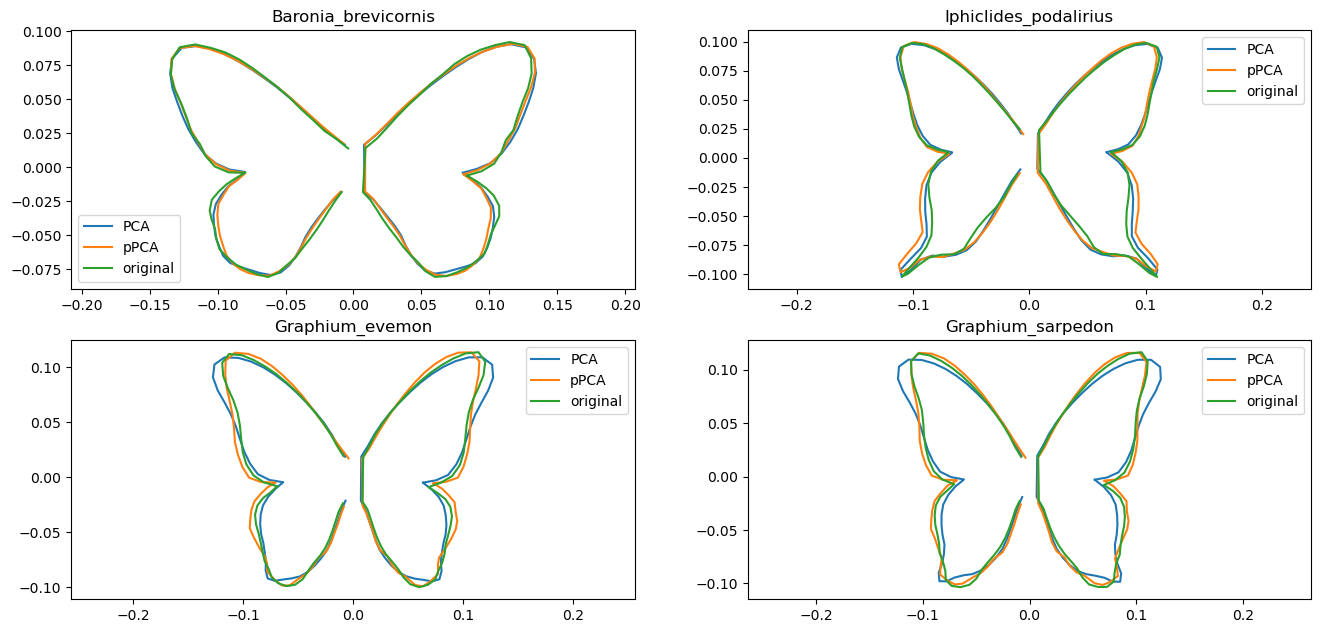
\includegraphics[scale=0.5]{recons-cropped.png}
        \caption{Sample of reconstructions with k=2}
    \end{center}
\end{figure}



\section{Algorithm runtime improvements}


\begin{lstlisting}
def design_matrix_slow(n, m):
    des = np.zeros((n * m, m))
    
    for i in range(n * m):
        for j in range(m):
            if (j - 1) * n < i >= j * n:
                des[i, j] = 1.
    
    return des
 


\end{lstlisting}


% used AI
\begin{lstlisting}
def design_matrix(n,m):
    des = np.zeros((n*m, m))
    i_indices = np.arange(n*m)
    j_indices = np.arange(m)
    # Use broadcasting to create a mask
    mask = (j_indices[:, None] * n <= i_indices) & (i_indices < (j_indices[:, None] + 1) * n)
    des[mask.T] = 1.0
    return des

\end{lstlisting}

\printbibliography

\end{document}
